\documentclass[border=3mm]{standalone}

\usepackage{tikz}



\usetikzlibrary{arrows,shapes.gates.logic.US,shapes.gates.logic.IEC,calc}
\begin{document}
\thispagestyle{empty}
\tikzstyle{branch}=[fill,shape=circle,minimum size=3pt,inner sep=0pt]

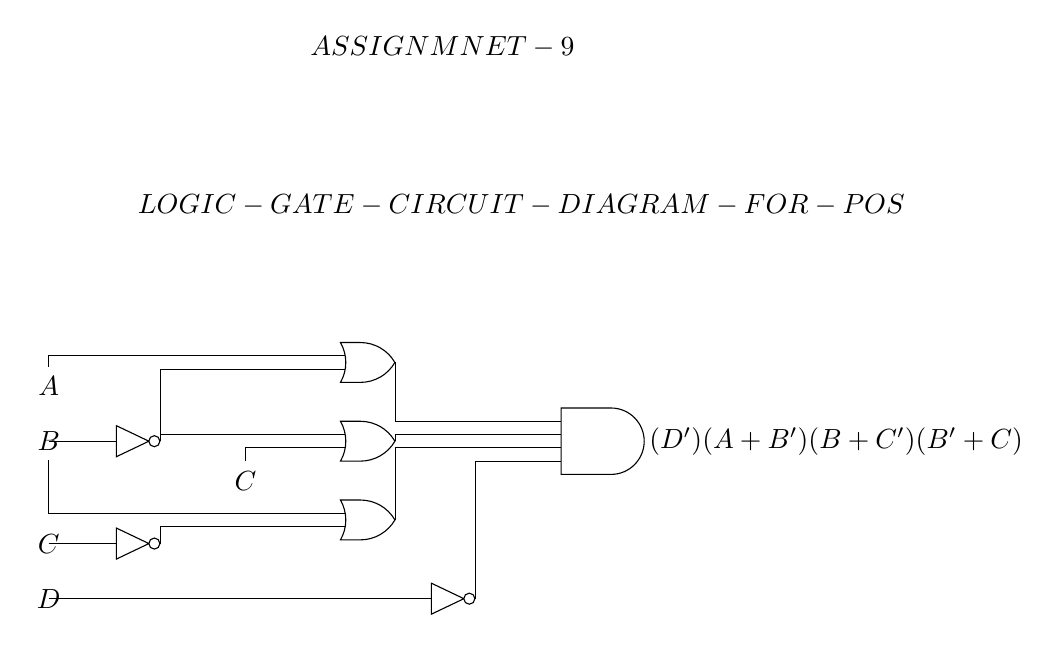
\begin{tikzpicture}[label distance=5mm]

     \node (x1) at (0,2) {$B$};
     \node (x2) at (0,0.7) {$C$};
     \node (x3) at (0,0) {$D$};
     \node (x4) at (2.5,1.5) {$C$};
     \node (x5) at (0,2.7) {$A$};   
     \node (x6) at (10,2) {$(D')(A+B')(B+C')(B'+C)$};
     \node (x7) at (5,7) {$ASSIGNMNET-9$};
     \node (x8) at (6,5) {$LOGIC-GATE-CIRCUIT-DIAGRAM-FOR-POS$};

     \node[not gate US, draw, rotate=0] at ($(x3)+(5,0)$) (Not1) {};
     \node[not gate US, draw, rotate=0] at ($(x2)+(1,0)$) (Not2) {};
     \node[not gate US, draw, rotate=0] at ($(x1)+(1,0)$) (Not3) {};
     
     \node[or gate US, draw, logic gate inputs=nn] at ($(x3)+(4,3)$) (Or1) {};
     \node[or gate US, draw, logic gate inputs=nn] at ($(x3)+(4,2)$) (Or2) {};
     \node[or gate US, draw, logic gate inputs=nn] at ($(x3)+(4,1)$) (Or3) {};
     \node[and gate US, draw, logic gate inputs=nnnn] at ($(7,2)$) (And1) {};

     \draw (Or1.output) |- (And1.input 1);
     \draw (Or2.output) |- (And1.input 2);
     \draw (Or3.output) |- (And1.input 3);
     \draw (Not1.output) |- (And1.input 4);
     \draw (Not2.output) |- (Or3.input 2);
     \draw (Not3.output) |- (Or2.input 1);
     \draw (Not3.output) |- (Or1.input 2);
     
 
     \draw (x1) |- (Not3.input);
     \draw (x2) |- (Not2.input);  
     \draw (x3) |- (Not1.input); 
     \draw (x4) |- (Or2.input 2);
     \draw (x1) |- (Or3.input 1);
     \draw (x5) |- (Or1.input 1);
     





\end{tikzpicture}


         

         


%    \end{questions}

\end{document}

